% Options for packages loaded elsewhere
\PassOptionsToPackage{unicode}{hyperref}
\PassOptionsToPackage{hyphens}{url}
\PassOptionsToPackage{dvipsnames,svgnames,x11names}{xcolor}
%
\documentclass[
  letterpaper,
  DIV=11,
  numbers=noendperiod]{scrartcl}

\usepackage{amsmath,amssymb}
\usepackage{iftex}
\ifPDFTeX
  \usepackage[T1]{fontenc}
  \usepackage[utf8]{inputenc}
  \usepackage{textcomp} % provide euro and other symbols
\else % if luatex or xetex
  \usepackage{unicode-math}
  \defaultfontfeatures{Scale=MatchLowercase}
  \defaultfontfeatures[\rmfamily]{Ligatures=TeX,Scale=1}
\fi
\usepackage{lmodern}
\ifPDFTeX\else  
    % xetex/luatex font selection
\fi
% Use upquote if available, for straight quotes in verbatim environments
\IfFileExists{upquote.sty}{\usepackage{upquote}}{}
\IfFileExists{microtype.sty}{% use microtype if available
  \usepackage[]{microtype}
  \UseMicrotypeSet[protrusion]{basicmath} % disable protrusion for tt fonts
}{}
\makeatletter
\@ifundefined{KOMAClassName}{% if non-KOMA class
  \IfFileExists{parskip.sty}{%
    \usepackage{parskip}
  }{% else
    \setlength{\parindent}{0pt}
    \setlength{\parskip}{6pt plus 2pt minus 1pt}}
}{% if KOMA class
  \KOMAoptions{parskip=half}}
\makeatother
\usepackage{xcolor}
\setlength{\emergencystretch}{3em} % prevent overfull lines
\setcounter{secnumdepth}{-\maxdimen} % remove section numbering
% Make \paragraph and \subparagraph free-standing
\ifx\paragraph\undefined\else
  \let\oldparagraph\paragraph
  \renewcommand{\paragraph}[1]{\oldparagraph{#1}\mbox{}}
\fi
\ifx\subparagraph\undefined\else
  \let\oldsubparagraph\subparagraph
  \renewcommand{\subparagraph}[1]{\oldsubparagraph{#1}\mbox{}}
\fi

\usepackage{color}
\usepackage{fancyvrb}
\newcommand{\VerbBar}{|}
\newcommand{\VERB}{\Verb[commandchars=\\\{\}]}
\DefineVerbatimEnvironment{Highlighting}{Verbatim}{commandchars=\\\{\}}
% Add ',fontsize=\small' for more characters per line
\usepackage{framed}
\definecolor{shadecolor}{RGB}{241,243,245}
\newenvironment{Shaded}{\begin{snugshade}}{\end{snugshade}}
\newcommand{\AlertTok}[1]{\textcolor[rgb]{0.68,0.00,0.00}{#1}}
\newcommand{\AnnotationTok}[1]{\textcolor[rgb]{0.37,0.37,0.37}{#1}}
\newcommand{\AttributeTok}[1]{\textcolor[rgb]{0.40,0.45,0.13}{#1}}
\newcommand{\BaseNTok}[1]{\textcolor[rgb]{0.68,0.00,0.00}{#1}}
\newcommand{\BuiltInTok}[1]{\textcolor[rgb]{0.00,0.23,0.31}{#1}}
\newcommand{\CharTok}[1]{\textcolor[rgb]{0.13,0.47,0.30}{#1}}
\newcommand{\CommentTok}[1]{\textcolor[rgb]{0.37,0.37,0.37}{#1}}
\newcommand{\CommentVarTok}[1]{\textcolor[rgb]{0.37,0.37,0.37}{\textit{#1}}}
\newcommand{\ConstantTok}[1]{\textcolor[rgb]{0.56,0.35,0.01}{#1}}
\newcommand{\ControlFlowTok}[1]{\textcolor[rgb]{0.00,0.23,0.31}{#1}}
\newcommand{\DataTypeTok}[1]{\textcolor[rgb]{0.68,0.00,0.00}{#1}}
\newcommand{\DecValTok}[1]{\textcolor[rgb]{0.68,0.00,0.00}{#1}}
\newcommand{\DocumentationTok}[1]{\textcolor[rgb]{0.37,0.37,0.37}{\textit{#1}}}
\newcommand{\ErrorTok}[1]{\textcolor[rgb]{0.68,0.00,0.00}{#1}}
\newcommand{\ExtensionTok}[1]{\textcolor[rgb]{0.00,0.23,0.31}{#1}}
\newcommand{\FloatTok}[1]{\textcolor[rgb]{0.68,0.00,0.00}{#1}}
\newcommand{\FunctionTok}[1]{\textcolor[rgb]{0.28,0.35,0.67}{#1}}
\newcommand{\ImportTok}[1]{\textcolor[rgb]{0.00,0.46,0.62}{#1}}
\newcommand{\InformationTok}[1]{\textcolor[rgb]{0.37,0.37,0.37}{#1}}
\newcommand{\KeywordTok}[1]{\textcolor[rgb]{0.00,0.23,0.31}{#1}}
\newcommand{\NormalTok}[1]{\textcolor[rgb]{0.00,0.23,0.31}{#1}}
\newcommand{\OperatorTok}[1]{\textcolor[rgb]{0.37,0.37,0.37}{#1}}
\newcommand{\OtherTok}[1]{\textcolor[rgb]{0.00,0.23,0.31}{#1}}
\newcommand{\PreprocessorTok}[1]{\textcolor[rgb]{0.68,0.00,0.00}{#1}}
\newcommand{\RegionMarkerTok}[1]{\textcolor[rgb]{0.00,0.23,0.31}{#1}}
\newcommand{\SpecialCharTok}[1]{\textcolor[rgb]{0.37,0.37,0.37}{#1}}
\newcommand{\SpecialStringTok}[1]{\textcolor[rgb]{0.13,0.47,0.30}{#1}}
\newcommand{\StringTok}[1]{\textcolor[rgb]{0.13,0.47,0.30}{#1}}
\newcommand{\VariableTok}[1]{\textcolor[rgb]{0.07,0.07,0.07}{#1}}
\newcommand{\VerbatimStringTok}[1]{\textcolor[rgb]{0.13,0.47,0.30}{#1}}
\newcommand{\WarningTok}[1]{\textcolor[rgb]{0.37,0.37,0.37}{\textit{#1}}}

\providecommand{\tightlist}{%
  \setlength{\itemsep}{0pt}\setlength{\parskip}{0pt}}\usepackage{longtable,booktabs,array}
\usepackage{calc} % for calculating minipage widths
% Correct order of tables after \paragraph or \subparagraph
\usepackage{etoolbox}
\makeatletter
\patchcmd\longtable{\par}{\if@noskipsec\mbox{}\fi\par}{}{}
\makeatother
% Allow footnotes in longtable head/foot
\IfFileExists{footnotehyper.sty}{\usepackage{footnotehyper}}{\usepackage{footnote}}
\makesavenoteenv{longtable}
\usepackage{graphicx}
\makeatletter
\def\maxwidth{\ifdim\Gin@nat@width>\linewidth\linewidth\else\Gin@nat@width\fi}
\def\maxheight{\ifdim\Gin@nat@height>\textheight\textheight\else\Gin@nat@height\fi}
\makeatother
% Scale images if necessary, so that they will not overflow the page
% margins by default, and it is still possible to overwrite the defaults
% using explicit options in \includegraphics[width, height, ...]{}
\setkeys{Gin}{width=\maxwidth,height=\maxheight,keepaspectratio}
% Set default figure placement to htbp
\makeatletter
\def\fps@figure{htbp}
\makeatother

\KOMAoption{captions}{tableheading}
\makeatletter
\makeatother
\makeatletter
\makeatother
\makeatletter
\@ifpackageloaded{caption}{}{\usepackage{caption}}
\AtBeginDocument{%
\ifdefined\contentsname
  \renewcommand*\contentsname{Table of contents}
\else
  \newcommand\contentsname{Table of contents}
\fi
\ifdefined\listfigurename
  \renewcommand*\listfigurename{List of Figures}
\else
  \newcommand\listfigurename{List of Figures}
\fi
\ifdefined\listtablename
  \renewcommand*\listtablename{List of Tables}
\else
  \newcommand\listtablename{List of Tables}
\fi
\ifdefined\figurename
  \renewcommand*\figurename{Figure}
\else
  \newcommand\figurename{Figure}
\fi
\ifdefined\tablename
  \renewcommand*\tablename{Table}
\else
  \newcommand\tablename{Table}
\fi
}
\@ifpackageloaded{float}{}{\usepackage{float}}
\floatstyle{ruled}
\@ifundefined{c@chapter}{\newfloat{codelisting}{h}{lop}}{\newfloat{codelisting}{h}{lop}[chapter]}
\floatname{codelisting}{Listing}
\newcommand*\listoflistings{\listof{codelisting}{List of Listings}}
\makeatother
\makeatletter
\@ifpackageloaded{caption}{}{\usepackage{caption}}
\@ifpackageloaded{subcaption}{}{\usepackage{subcaption}}
\makeatother
\makeatletter
\@ifpackageloaded{tcolorbox}{}{\usepackage[skins,breakable]{tcolorbox}}
\makeatother
\makeatletter
\@ifundefined{shadecolor}{\definecolor{shadecolor}{rgb}{.97, .97, .97}}
\makeatother
\makeatletter
\makeatother
\makeatletter
\makeatother
\ifLuaTeX
  \usepackage{selnolig}  % disable illegal ligatures
\fi
\IfFileExists{bookmark.sty}{\usepackage{bookmark}}{\usepackage{hyperref}}
\IfFileExists{xurl.sty}{\usepackage{xurl}}{} % add URL line breaks if available
\urlstyle{same} % disable monospaced font for URLs
\hypersetup{
  pdftitle={TP2:Étude de l'effet de la satisfaction démocratique sur le niveau de participation à des organismes politiques (Option 2).},
  pdfauthor={Egemen Akyildiz},
  colorlinks=true,
  linkcolor={blue},
  filecolor={Maroon},
  citecolor={Blue},
  urlcolor={Blue},
  pdfcreator={LaTeX via pandoc}}

\title{TP2:Étude de l'effet de la satisfaction démocratique sur le
niveau de participation à des organismes politiques (Option 2).}
\author{Egemen Akyildiz}
\date{}

\begin{document}
\maketitle
\ifdefined\Shaded\renewenvironment{Shaded}{\begin{tcolorbox}[breakable, boxrule=0pt, borderline west={3pt}{0pt}{shadecolor}, sharp corners, interior hidden, frame hidden, enhanced]}{\end{tcolorbox}}\fi

\hypertarget{introduction}{%
\subsection{Introduction}\label{introduction}}

Il y a eu deux élections au Canada au niveau fédéral en 2019 et en 2021.
Dans les deux cas, le premier ministre sortant Justin Trudeau les a
emporté. À l'aide de deux sondages trouvés sur le site web Odesi.ca qui
ont eu lieu durant les deux campagnes électorales nous allons nous poser
une question. Le niveau de satisfaction avec la démocratie au Canada et
le niveau de participation politique, plus précisément le volontariat ou
l'association aux groupes ou organisations a-t-il un lien? En d'autres
mots, le niveau de satisfaction avec la démocratie affecte-t-il la
participation politique autre que le vote.

C'est une possible corrélation que nous pourrions trouver intéressant
d'étudier de plus près. Dans toutes les démocraties du monde, les
citoyens sont de moins en moins positifs au sujet de ce type de régime.
Une certaine désillusion face au modèle démocratique règne. Ce manque de
satisfaction pourrait mener à une plus faible participation politique,
ce qui augmenterait aussi le manque de confiance envers le modèle
démocratique. Il se pourrait qu'il y ait un cercle vicieux, et nous
désirons analyser le potentiel d'existence de ce lien.

Les données que nous allons utiliser viennent comme nous l'avons dit
plus haut de deux sondages élaborés durant les campagnes de chaque
élection, 2019 et 2021. Ces sondages viennent d'Élections Canada, agence
non-partisane de l'État. Les réponses récoltés dans ces sondages seront
utilisées. Nous avons utilisé deux sondages pour pouvoir avoir un plus
grand nombre de répondants. Malgré le fait que les sondages ont été fait
à deux ans d'écart, nous estimons pour simplifier les choses qu'il ne
s'est pas passé d'évènements assez important au sujet de la démocratie.
Nous rappelons que l'évènement du freedom convoy s'est déroulé en 2022.

\hypertarget{donnuxe9es-et-muxe9thode}{%
\subsection{Données et méthode}\label{donnuxe9es-et-muxe9thode}}

Les données de sondage sont de type catégoriel. Les deux sondages ont un
très grand nombre de participants. Il y a dans le premier sondage, celui
de 2019, 37822 répondants et 633 variables. Le deuxième sondage de
l'élection de 2021 a un total de 20968 répondants et 1090 variables. Les
variables catégorielles que nous avons extrait des deux sondages sont de
type ordinal et exactement les mêmes. La variable satisfaction a 5
réponses possibles comme suit: 1 = Très satisfait, 2 = Assez satisfait,
3 = Pas très satisfait, 4 = Insatisfait, 5 = Je ne sais pas/ne veux pas
répondre. La variable participation, qui demande le niveau de
participation dans les douzes derniers mois, a les suivantes: 1 =
Jamais, 2 = Une fois, 3 = Quelques fois, 4 = Plus de cinq fois, 5 = Je
ne sais pas/ne veux pas répondre. Bien évidemment, le sondage canadien a
été fait en anglais mais nous prenons la liberté de traduire les termes
en français dès maintenant.

Parlons maintenant du processus de nettoyage, uniformisation et ainsi de
suite. Tout d'abord nous avons téléchargé les bibliothèque ``dplyr'' et
``ggplot2'', le premier pour certaines commandes que nous ne pouvions
pas nous en passer, la deuxième pour la création de notre graphique.

Ensuite nous avons téléchargé les bases de données que nous avions
ultérieurement placé dans le fichier du tp2. La commande ``read.csv'' a
été mobilisé à cette fin pour nos deux bases de données.

Les deux bases de données téléchargé sur Rstudio, nous avons modifié
quelques données. Nous avons changé les noms des variables à l'aide de
la commande ``rename'' pour qu'elles ne soient pas que des lettres et
chiffres sans sens. Et nous avons supprimé la réponse 5 des deux
variables avec la commande ``filter'' car elles ne nous aidaient pas
dans l'élaboration du travail. Ce sont des valeurs que l'on pourrait
qualifier de polluante. Et nous nous sommes assuré avec la commande
``na.omit()'' qu'il ne se trouvait plus de lignes avec des valeurs
manquantes en les supprimant. Tout cela pour nos deux bases de données.

Ensuite nous avons combiné nos deux bases dans une seule avec la
commande ``bind.rows()'' qui fusionnent les lignes des deux bases de
données.

Par la suite, nous avons transformé nos variables ordinales en variables
numériques afin d'aider à la fabrication de notre graphique grâce à la
commande ``mutate()'' et ``as.numeric''. Ceci est utile dans
l'éventualité que nous voulons faire des calculs d'analyse. Nous avons
bien entendu appliqué la commande ``filter()'' pour nous assurer qu'il
n'y avait pas de lignes avec des valeurs manquantes, ce qui pourrait
ruiner notre résultat.

Ensuite pour pouvoir créer un graphique le plus lisible possible, nous
avons créer une nouvelle colonne dans notre base de données qui lie les
valeurs numériques de la variable ``satisfaction'' aux terme décrits
plus tôt: ``Très satisfait'', ``Assez satisfait'' et ainsi de suite.
Tout cela avec la commande ``factor()'', et les arguments ``levels()'',
reliés aux chiffres et ``labels()'' reliées aux étiquettes. De plus,
nous avons aussi utilisé ``participation\_labels \textless- c()'' pour
créer un vecteur qui lie les étiquettes de la variable participation
(Jamais, Une fois etc.) pour pouvoir éclaircir notre graphique fait avec
ggplot2 en étiquetant les chiffres de la variable ``participation'' dans
la légende.

\hypertarget{ruxe9sultats-et-graphique}{%
\subsection{Résultats et graphique}\label{ruxe9sultats-et-graphique}}

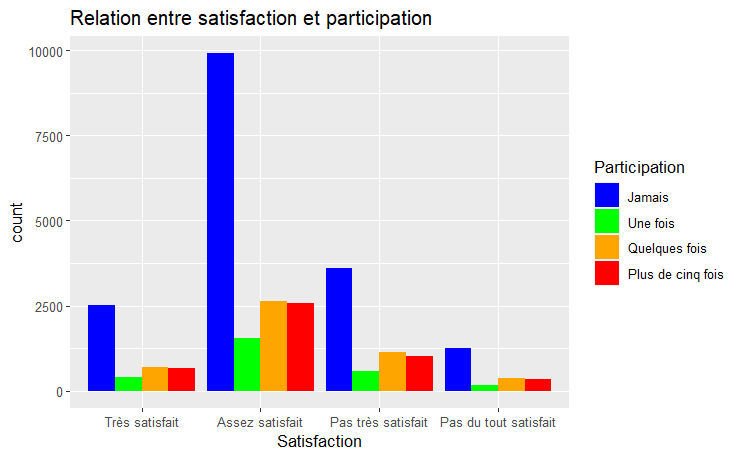
\includegraphics{graphiqueTP2.png}

Les résultats ne sont pas très impressionants. Nous voulons tout d'abord
mentionner le nombre d'observations dans chaque base et le nombre de
variable. La base de données de 2019 après nettoyage contient 9675
observations et 2 variables tandis que celle de 2021 contient 19804
observations et 2 variables. Bien entendu, les 2 variables sont les
mêmes dans les deux cas. Nous avions supprimé la cinquième réponse de
chaque variable des deux bases. La base de données combinée a un total
de 29479 observations avec 3 variables. Il est important de noter que la
troisième variable n'est qu'une version en mots de la variable
``satisfaction'', ce qui nous était utile pour le graphique. Donc nous
pouvons tout juste dire qu'en réalité nous n'avons que deux variables
pour la base de données combiné, que nous avons nommé
``combined\_data''. Les variables viennent des sondages élaborés par
Élections Canada durant les campagnes présidentielles.

Comme nous pouvons le voir dans le graphique la plus grande part des
répondants sont assez satisfaits avec la démocratie au Canada. Mais le
fait que le nombre de gens très satisfaits de la démocratie soit aussi
proche du nombre de gens qui ne sont pas du tout satisfait est très
inquiétant pour le futur de notre pays. Le deuxième plus grand nombre
d'observations vient des gens qui ne sont pas très satisfaits, encore un
mauvais présage. Le nombre de gens qui n'ont pas du tout participé à un
organisme politique est largement majoritaire au reste. Extrêmement peu
de gens n'ont participé qu'une seule fois. Et il se trouve que le nombre
de gens qui y ont participé quelques fois à cinq fois et plus est très
similaire. Proportionnellement parlant, le graphique nous montre que le
niveau de participation politique est relativement le même pour tout les
niveaux de satisfaction. Ceci est plutôt étonnant. Nous nous attendions
à une corrélation claire est nette mais nous ne l'avons pas obtenu.

\hypertarget{annexe}{%
\subsubsection{Annexe}\label{annexe}}

\begin{Shaded}
\begin{Highlighting}[]
\FunctionTok{library}\NormalTok{(dplyr)}
\end{Highlighting}
\end{Shaded}

\begin{verbatim}
Warning: package 'dplyr' was built under R version 4.3.2
\end{verbatim}

\begin{verbatim}

Attaching package: 'dplyr'
\end{verbatim}

\begin{verbatim}
The following objects are masked from 'package:stats':

    filter, lag
\end{verbatim}

\begin{verbatim}
The following objects are masked from 'package:base':

    intersect, setdiff, setequal, union
\end{verbatim}

\begin{Shaded}
\begin{Highlighting}[]
\FunctionTok{library}\NormalTok{(ggplot2)}
\end{Highlighting}
\end{Shaded}

\begin{verbatim}
Warning: package 'ggplot2' was built under R version 4.3.2
\end{verbatim}

\begin{Shaded}
\begin{Highlighting}[]
\NormalTok{data\_2019 }\OtherTok{\textless{}{-}} \FunctionTok{read.csv}\NormalTok{(}\StringTok{"C:/Users/Gul/Desktop/UDM\_SCI\_PO/Hiver\_2024/FAS1001/fas\_1001\_akyildiz/\_tp/\_tp2/data2019.csv"}\NormalTok{) }\CommentTok{\#data 2019}
\NormalTok{data\_2021 }\OtherTok{\textless{}{-}} \FunctionTok{read.csv}\NormalTok{(}\StringTok{"C:/Users/Gul/Desktop/UDM\_SCI\_PO/Hiver\_2024/FAS1001/fas\_1001\_akyildiz/\_tp/\_tp2/data2021.csv"}\NormalTok{) }\CommentTok{\#data 2021}
\end{Highlighting}
\end{Shaded}

\begin{Shaded}
\begin{Highlighting}[]
\NormalTok{data\_2019\_clean }\OtherTok{\textless{}{-}}\NormalTok{ data\_2019 }\SpecialCharTok{|\textgreater{}}
\FunctionTok{select}\NormalTok{(pes19\_dem\_sat, cps19\_volunteer   ) }\SpecialCharTok{|\textgreater{}}
    \FunctionTok{rename}\NormalTok{(}\AttributeTok{satisfaction =}\NormalTok{ pes19\_dem\_sat, }\AttributeTok{participation =}\NormalTok{ cps19\_volunteer) }\SpecialCharTok{|\textgreater{}}
    \FunctionTok{filter}\NormalTok{(satisfaction }\SpecialCharTok{!=} \StringTok{"5"}\NormalTok{) }\SpecialCharTok{|\textgreater{}}
    \FunctionTok{filter}\NormalTok{(participation }\SpecialCharTok{!=} \StringTok{"5"}\NormalTok{) }\SpecialCharTok{|\textgreater{}}
  \FunctionTok{na.omit}\NormalTok{() }
\end{Highlighting}
\end{Shaded}

\begin{Shaded}
\begin{Highlighting}[]
\NormalTok{data\_2021\_clean }\OtherTok{\textless{}{-}}\NormalTok{ data\_2021 }\SpecialCharTok{|\textgreater{}}
  \FunctionTok{select}\NormalTok{(cps21\_demsat   , cps21\_volunteer) }\SpecialCharTok{|\textgreater{}}
    \FunctionTok{rename}\NormalTok{(}\AttributeTok{satisfaction =}\NormalTok{ cps21\_demsat,}
         \AttributeTok{participation =}\NormalTok{ cps21\_volunteer) }\SpecialCharTok{|\textgreater{}}
    \FunctionTok{filter}\NormalTok{(satisfaction }\SpecialCharTok{!=} \StringTok{"5"}\NormalTok{) }\SpecialCharTok{|\textgreater{}}
    \FunctionTok{filter}\NormalTok{(participation }\SpecialCharTok{!=} \StringTok{"5"}\NormalTok{) }\SpecialCharTok{|\textgreater{}}
  \FunctionTok{na.omit}\NormalTok{() }
\end{Highlighting}
\end{Shaded}

\begin{Shaded}
\begin{Highlighting}[]
\NormalTok{combined\_data }\OtherTok{\textless{}{-}} \FunctionTok{bind\_rows}\NormalTok{(data\_2019\_clean, data\_2021\_clean)}
\end{Highlighting}
\end{Shaded}

\begin{Shaded}
\begin{Highlighting}[]
\NormalTok{combined\_data }\OtherTok{\textless{}{-}}\NormalTok{ combined\_data }\SpecialCharTok{\%\textgreater{}\%}
  \FunctionTok{mutate}\NormalTok{(}\AttributeTok{satisfaction =} \FunctionTok{as.numeric}\NormalTok{(satisfaction),}
         \AttributeTok{participation =} \FunctionTok{as.numeric}\NormalTok{(participation)) }\SpecialCharTok{\%\textgreater{}\%}
  \FunctionTok{filter}\NormalTok{(}\SpecialCharTok{!}\FunctionTok{is.na}\NormalTok{(satisfaction) }\SpecialCharTok{\&} \SpecialCharTok{!}\FunctionTok{is.na}\NormalTok{(participation))}
\end{Highlighting}
\end{Shaded}

\begin{Shaded}
\begin{Highlighting}[]
\NormalTok{combined\_data}\SpecialCharTok{$}\NormalTok{satisfaction\_label }\OtherTok{\textless{}{-}} \FunctionTok{factor}\NormalTok{(combined\_data}\SpecialCharTok{$}\NormalTok{satisfaction,}
                                           \AttributeTok{levels =} \FunctionTok{c}\NormalTok{(}\DecValTok{1}\NormalTok{, }\DecValTok{2}\NormalTok{, }\DecValTok{3}\NormalTok{, }\DecValTok{4}\NormalTok{),}
                                           \AttributeTok{labels =} \FunctionTok{c}\NormalTok{(}\StringTok{"Très satisfait"}\NormalTok{, }\StringTok{"Assez satisfait"}\NormalTok{, }\StringTok{"Pas très satisfait"}\NormalTok{, }\StringTok{"Pas du tout satisfait"}\NormalTok{))}

\NormalTok{participation\_labels }\OtherTok{\textless{}{-}} \FunctionTok{c}\NormalTok{(}\StringTok{"Jamais"}\NormalTok{, }\StringTok{"Une fois"}\NormalTok{, }\StringTok{"Quelques fois"}\NormalTok{, }\StringTok{"Plus de cinq fois"}\NormalTok{)}
\end{Highlighting}
\end{Shaded}

\begin{Shaded}
\begin{Highlighting}[]
\FunctionTok{ggplot}\NormalTok{(combined\_data, }\FunctionTok{aes}\NormalTok{(}\AttributeTok{x =}\NormalTok{ satisfaction\_label, }\AttributeTok{fill =} \FunctionTok{as.factor}\NormalTok{(participation))) }\SpecialCharTok{+}
  \FunctionTok{geom\_bar}\NormalTok{(}\AttributeTok{position =} \StringTok{"dodge"}\NormalTok{) }\SpecialCharTok{+}
  \FunctionTok{labs}\NormalTok{(}\AttributeTok{title =} \StringTok{"Relation entre satisfaction et participation"}\NormalTok{,}
       \AttributeTok{x =} \StringTok{"Satisfaction"}\NormalTok{, }
       \AttributeTok{fill =} \StringTok{"Participation"}\NormalTok{) }\SpecialCharTok{+}
  \FunctionTok{scale\_fill\_manual}\NormalTok{(}\AttributeTok{values =} \FunctionTok{c}\NormalTok{(}\StringTok{"1"} \OtherTok{=} \StringTok{"blue"}\NormalTok{, }\StringTok{"2"} \OtherTok{=} \StringTok{"green"}\NormalTok{, }\StringTok{"3"} \OtherTok{=} \StringTok{"orange"}\NormalTok{, }\StringTok{"4"} \OtherTok{=} \StringTok{"red"}\NormalTok{),}
                    \AttributeTok{labels =}\NormalTok{ participation\_labels)}
\end{Highlighting}
\end{Shaded}

\begin{figure}[H]

{\centering 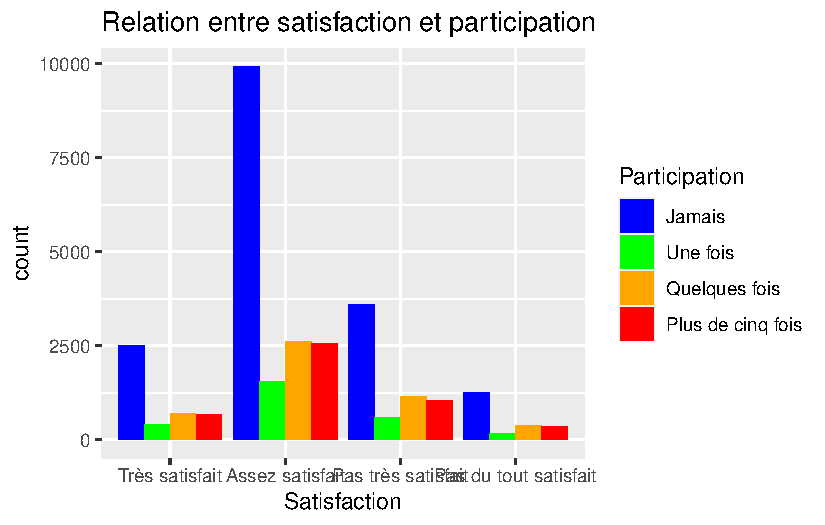
\includegraphics{TP2Akyildiz_files/figure-pdf/unnamed-chunk-8-1.pdf}

}

\end{figure}



\end{document}
